\section{Data Preprocessing}\label{data_preprocessing}

Data preprocessing is a vital step in the data mining process, particularly in the context of deep learning for image classification. This step involves techniques such as image augmentation, affine transformations, and resizing, which are essential for enhancing model performance. For this project, preprocessing is applied to the provided dataset (dataset\_19) to ensure it is suitable for the brain tumor classification task. The specific steps involved in the preprocessing of this dataset are outlined below.

\subsection{Dataset}\label{dataset_given}

The dataset, referred to as dataset\_19, comprises a folder containing four subfolders, each representing a different class of brain tumors. Each subfolder includes 120 MRI images of varying sizes. The dataset distribution is illustrated in Figure \ref{fig:data_distribution}.

\begin{figure}[H]
  \begin{center}
    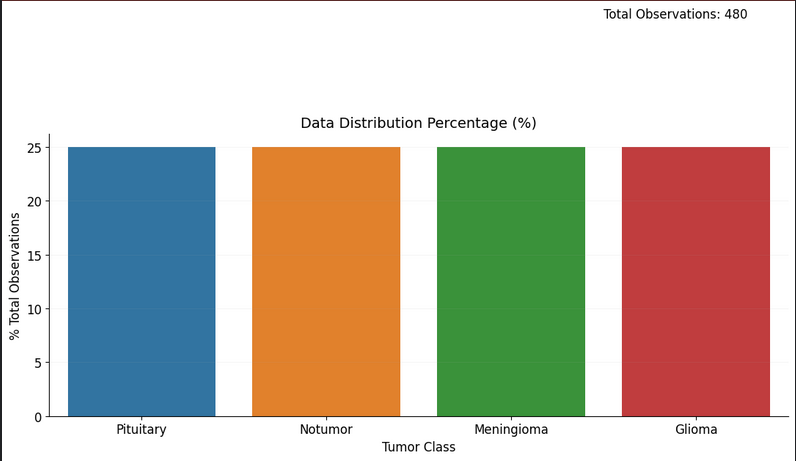
\includegraphics[width=0.95\textwidth]{Exploration/data_distribution.png}
  \end{center}
  \caption{Distribution of images in dataset\_19.}\label{fig:data_distribution}
\end{figure}

To prepare the dataset for the classification task, it is preprocessed and subsequently divided into training and validation sets, with the training set comprising 80\% of the data and the validation set 20\%. This split is shown in Figure \ref{fig:data_split}. The training set is used to train the model, while the validation set is used to evaluate its performance.

\begin{figure}[H]
  \begin{center}
    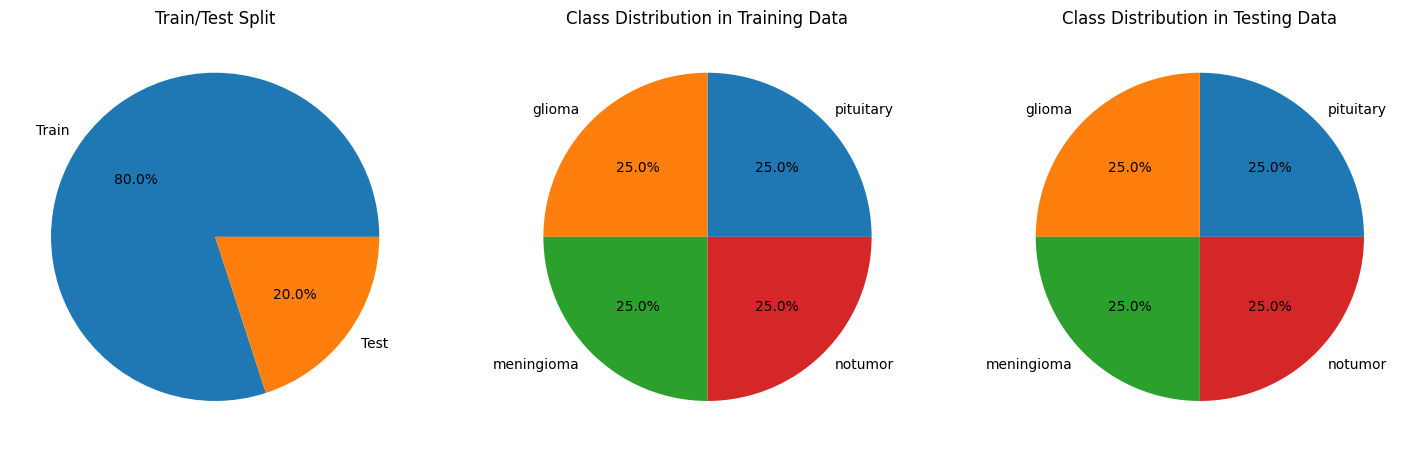
\includegraphics[width=0.95\textwidth]{Exploration/data_split.png}
  \end{center}
  \caption{Splitting the dataset into training and validation sets.}\label{fig:data_split}
\end{figure}

Image preprocessing is essential to enable models to focus on the region of interest, namely the brain, while reducing background noise and irrelevant features. This process involves converting images to grayscale, applying Gaussian blur, and performing thresholding and morphological operations to refine image quality. By cropping around the largest contour, which is likely the brain, this step highlights critical anatomical features and enhances model generalization, ultimately leading to more accurate tumor classification.

\begin{figure}[H]
  \begin{center}
    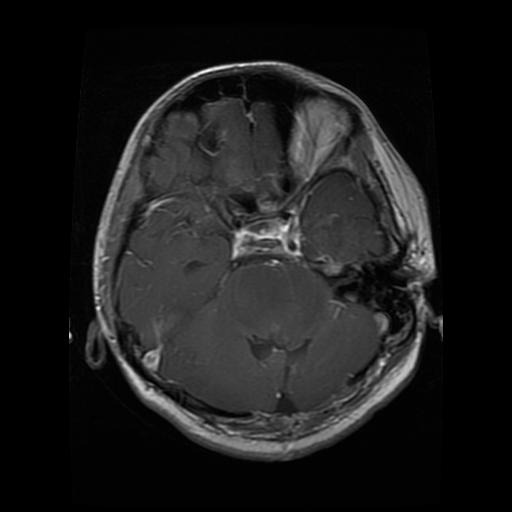
\includegraphics[width=0.3\textwidth]{Exploration/Te-gl_0010.jpg}
    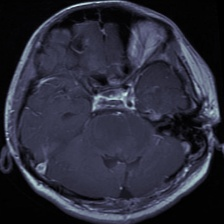
\includegraphics[width=0.3\textwidth]{Exploration/Te-gl_0010_preprocessed.jpg}
  \end{center}
  \caption{Cropping the MRI image along its contour.}\label{fig:image_cropping}
\end{figure}

Image augmentation is then performed using the \texttt{ImageDataGenerator} class from the Keras library. This technique artificially increases the dataset size by applying various transformations to the images, thus improving model performance by providing more training data. The \texttt{ImageDataGenerator} class offers several parameters for image augmentation.

The preprocessing pipeline involves initially performing horizontal flips on the images, followed by random rotations. Each image is then normalized by dividing pixel values by 255. After these transformations, the dataset is split into training and validation sets as previously described.

\subsection{Summary and Justifications}

Given the relatively small size of dataset\_19 (480 images in total), data augmentation is crucial for enhancing the dataset's variability and improving the model's generalization capabilities. Flipping images horizontally is justified based on the anatomical symmetry of the brain's hemispheres, allowing for effective augmentation without misrepresenting tumor locations \cite{nalepa_data_2019}. This technique increases the diversity of the training data, which is particularly important given the limited size of the dataset compared to larger datasets, such as those used in the BraTS competition.

Similarly, random rotations are applied since brain images can be rotated in various directions, further increasing the dataset's variability and aiding in model training. The augmentation strategies, including horizontal flipping and random rotations, are essential for compensating for the smaller dataset size by exposing the model to a wider variety of image orientations and perspectives. This approach helps create a more robust model capable of accurately classifying brain tumors despite the limited amount of original training data.

